\documentclass[letterpaper, 12pt]{article}
\usepackage[top=2cm,bottom=1cm,left=0.75in,right=0.75in,headheight=17pt, 
includehead,includefoot,
heightrounded, % to avoid spurious underfull messages
]{geometry}
\addtolength{\topmargin}{-.25in}
\usepackage{fancyhdr}
\pagestyle{fancy}
\usepackage{graphicx}
\usepackage{lastpage}
\usepackage{gensymb}
\usepackage{qrcode}

\begin{document}
\fancyhead[l]{	\includegraphics[height=1cm]{"../../Templates/Year C/club".png} Name:}
\fancyhead[r]{Due Date \hspace{ 1in} \vspace{.1in} }
\cfoot{\thepage\ of \pageref{LastPage}}
	

	
\begin{center}Assignment 5.03: Magnetic Induction
\end{center}

\begin{enumerate}




	\item A magnetic field is directed into the page.  There is a circular loop of wire with radius 0.25m in the plane of the page.  The magnetic field strength is increasing at a rate of 0.1 T/s.
	
\begin{enumerate}
	\item Does the induced current flow in a clockwise or counterclockwise direction?  Explain your reasoning.  
	
	\vspace{.75in}
	\item What is the magnitude of the induced EMF? 
\end{enumerate}

	\vspace{.75in}
	
		\item A magnetic field is directed out of the page, and is changing in strength.  There is a square-shaped piece of wire with each side having a length of 0.25 m.  The current induced in the wire is 0.2 Amps in a counterclockwise direction.  The resistance of the wire is $1 \Omega$.
	\begin{enumerate}
		\item Is the magnetic field getting stronger or weaker? Explain your reasoning.
		\vspace{.75in}
		\item At what rate is the magnetic field changing?
	\end{enumerate}
	
	\vspace{.75in}
	
		\item An equilateral triangle is oriented in the plane of the page.  A magnetic field is changing at a rate of 2 T/s, directed into the page.  The current that flows in the triangle is 1.5A and the resistance of the triangle is $2\Omega$. 
		\begin{enumerate}
			\item Does the induced current flow clockwise or counterclockwise?
			\vspace{0.75in}
			\item What is the length of the sides of the equilateral triangle?
		\end{enumerate}
		


	
	\vspace{1in}
		\item A hollow rectangle of metal is attached to all-plastic wheels.  As shown in the diagram, it then rolls to the right at a speed of 0.75 m/s, into a region of magnetic field. The strength of magnetic field is 2T.
		\begin{center}
				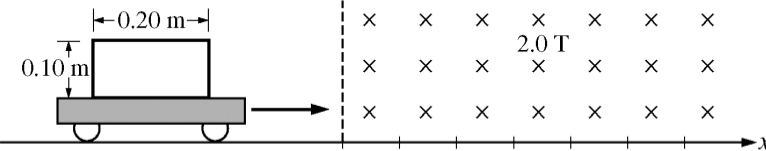
\includegraphics[height=.5in]{inductioncard.png}
		\end{center}
		\begin{enumerate}
			\item When the front edge of the cart has entered the magnetic field, but the back edge has not, what direction does current flow in the wire?
			\vspace{0.5in}
			\item The resistance of the rectangle is 0.2A.  What is the current in the wire?
			\vspace{0.5in}
			\item Calculate the force exerted on the cart as it enters the magnetic field.
			\vspace{0.5in}
			\item What is the force exerted on the cart when it is completely in the magnetic field?
			\vspace{0.5in}
		\end{enumerate}
	
	
		\item Induction stoves work by generating a rapidly oscillating magnetic field.  This causes current to flow in a ferromagnetic pot above it.  As current flows, resistive losses due to Ohm's Law cause the pot to heat up.  Suppose a magnetic field oscillates from 0.01 T to -0.01 T at a rate of 24 kHz.   
	\begin{enumerate}
		\item Determine the average rate of change of the magnetic field.  
		\vspace{.5in}
		\item If a frying pan is a circle with a radius of 8cm, what is the EMF induced in the pan?
			\vspace{.5in}
		\item Determine the power that is delivered to the pan if its resistance is 0.25 $\Omega$.
			\vspace{.5in}
		\item If the frying pan is made of Cast Iron ($ c = 450 \frac{J} {kg  \degree C}$), and has a mass of 0.6 kg, how long would it take to heat up from 20$\degree$C to 100$\degree$C
		
		
	\end{enumerate}
	
	\vspace{1in}

	
\end{enumerate}
 



\end{document}
